\begin{frame}{}
  \LARGE Safety, Ethics, and Control
\end{frame}

\begin{frame}{Safety in Agentic Systems}
  \begin{itemize}
    \item[\textcolor{red}{$\triangleright$}] \textbf{Risks:}
    \begin{itemize}
      \item Autonomous actions without human oversight
      \item Errors in tool or API use
      \item Prompt injection or goal hijacking
      \item Recursive self-improvement without constraints
    \end{itemize}
    \vspace{1em}
    \item[\textcolor{red}{$\triangleright$}] \textbf{Mitigations:}
    \begin{itemize}
      \item Approval-based execution: a person confirms a consequential action before the runtime executes it
      \item Guardrails: separate classifiers that screen the agent's inputs and outputs for injection
        attempts and policy violations
      \item Explainability (XAI) for agent decisions
    \end{itemize}
    \vspace{0.4em}
    \item[] {\small Each of these, and the threat model behind it, is treated in full later in the course.}
  \end{itemize}
\end{frame}

\begin{frame}{Governance Concerns Reported by Technology Leaders}
  \begin{figure}
    \centering
    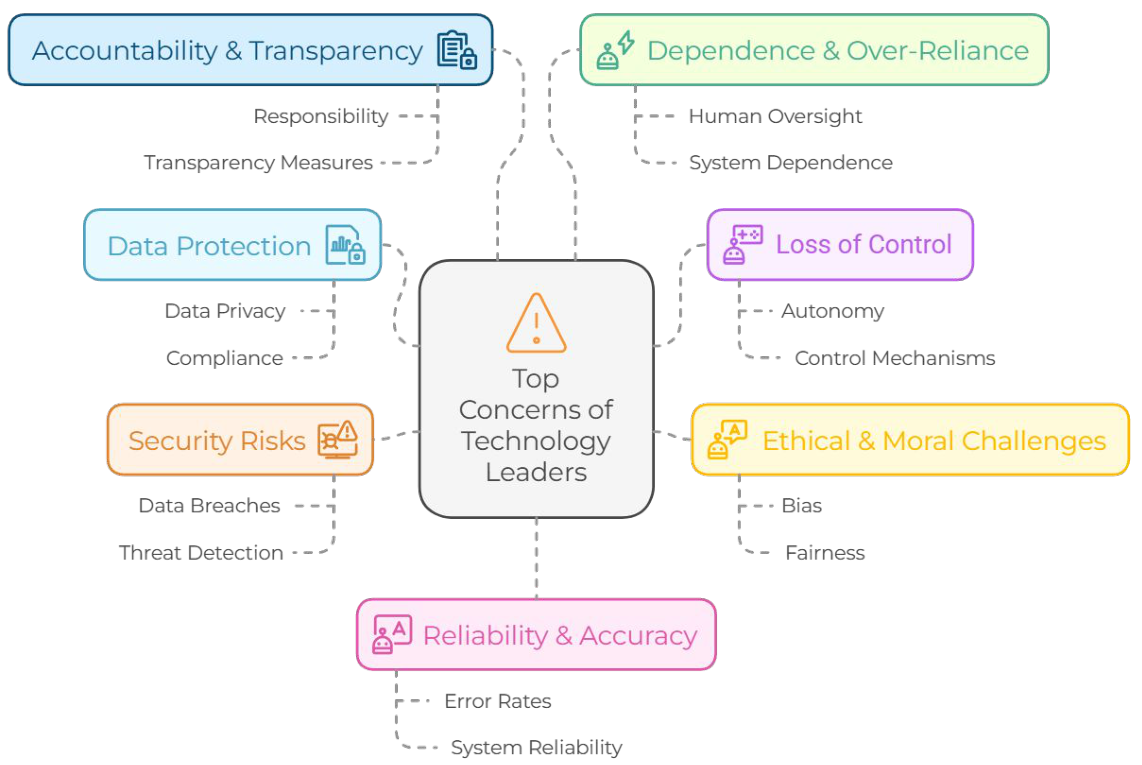
\includegraphics[width=0.8\textwidth,height=0.72\textheight,keepaspectratio]{images/agentic-ai/agentic_ai_governance_concerns.png}
    \caption*{\scriptsize Source: I.~Katusic, ``Top 7 Concerns of Technology Leaders That Implemented Agentic
    AI'', CTO Academy, 2025.}
  \end{figure}
\end{frame}

\begin{frame}{Multi-Agent Architectures}
  \begin{center}
    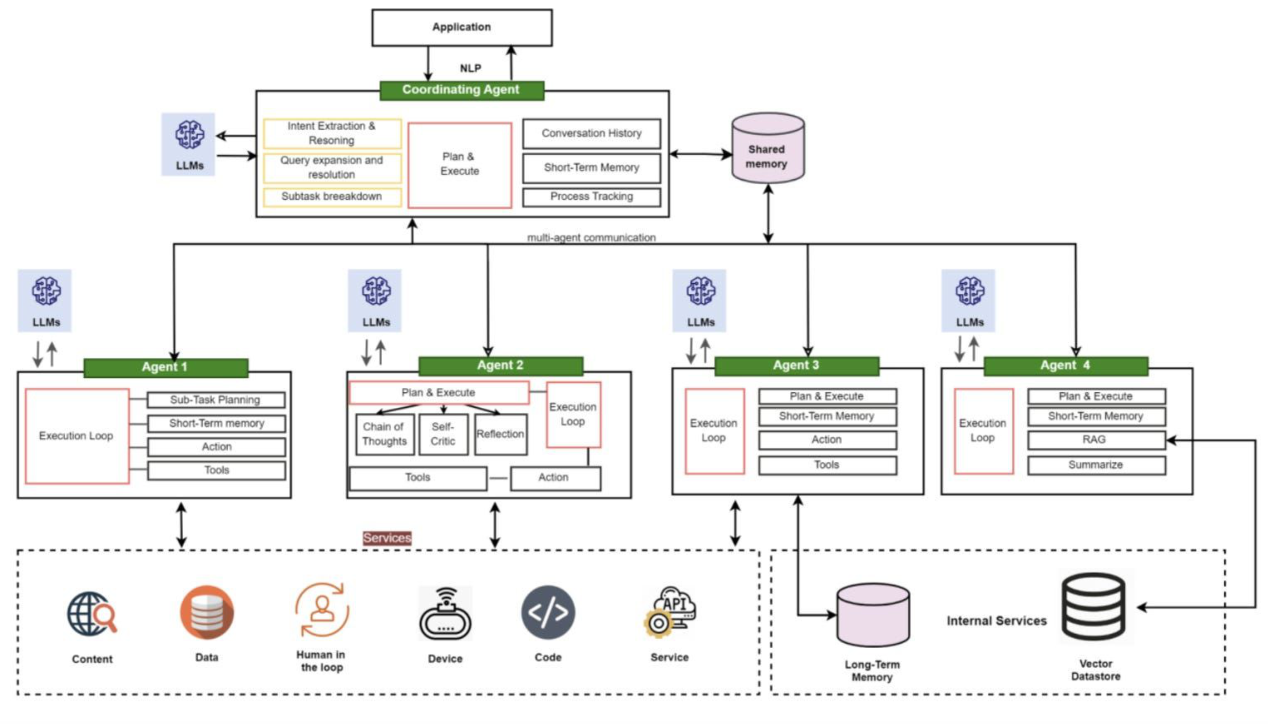
\includegraphics[width=0.85\textwidth,height=0.7\textheight,keepaspectratio]{images/agentic-ai/agentic_multiagent_coordination_architecture.png}
  \end{center}
  {\small
  An example multi-agent architecture built from specialised agents. Specialisation is one agentic
  pattern among several, and which pattern fits depends on the use case.\par}
  \vspace{0.3em}
  {\scriptsize
  Source: OWASP GenAI Security Project, ``Agentic AI -- Threats and Mitigations'', Agentic Security
  Initiative, v1.1 (December 2025), p.~10.\par}
\end{frame}


\begin{frame}{Ethics and Control}
  \begin{figure}
    \centering
    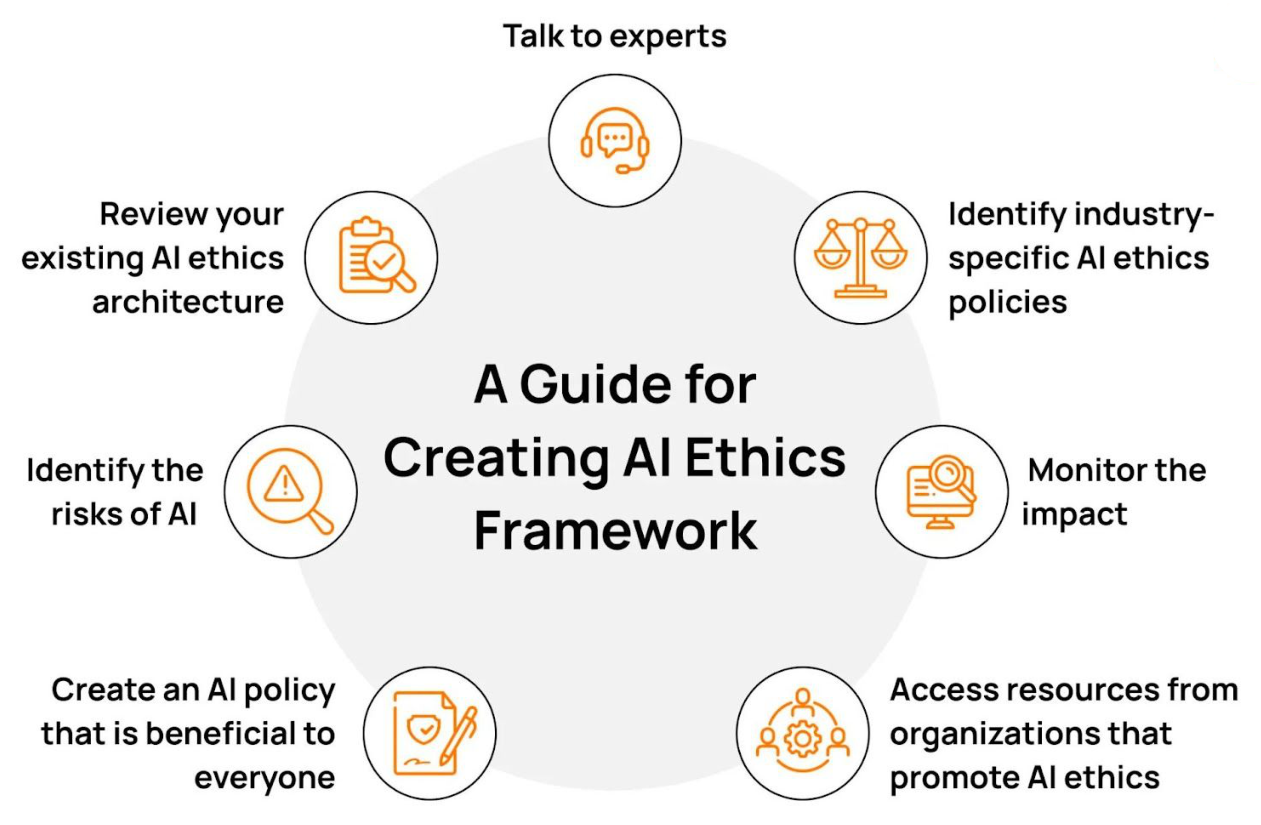
\includegraphics[width=0.8\textwidth,height=0.72\textheight,keepaspectratio]{images/agentic-ai/agentic_ai_ethics_framework_guide.png}
    \caption*{\scriptsize Source: P.~Parsani, ``How to Create an AI Ethics Framework for your Company?'',
    Cut the SaaS, 2024.}
  \end{figure}
\end{frame}

\begin{frame}{Ethics and Control}
  \begin{itemize}
    \item \textcolor{red}{Alignment:} Are agents acting in users' interests?
    \item \textcolor{red}{Accountability:} Who is responsible for AI actions?
    \item \textcolor{red}{Control:} Can humans override or audit decisions?
  \end{itemize}
  \vspace{1em}
  \textbf{Key Areas:}
  \begin{itemize}
    \item Fairness in multimodal data
    \item Bias amplification (vision + language)
    \item Transparency in decision-making
  \end{itemize}
\end{frame}
